\chapter{Outer Tracker Luminometer}

The CMS Phase II Outer Tracker system will provide a source of high rate physics objects: L1 track stubs,
due to its designed architecture which sends these objects to the L1 track reconstruction system at full 40 MHz frequency~\cite{CERN-LHCC-2017-009}.
Studies of CMS Phase II simulations show excellent linearity in the counting of these objects up to pile-up of 200.
Both of these properties make this an excellent candidate for a precision luminometer.
In the following sections, the detector layout, a preliminary design of the data acquisition system, and expected perfomace are described.


\section{Detector Layout }
- Description of the Outer Tracker layout (Layer 6)\\

- track stub objects

\section{Track Stub Counting and Data Acquisition}
- OT backend \\ 
- track stub histogramming \\
- data transfer 

\section{Expected Performance}
- Rates\\
- linearity \\
- statistical precision

\clearpage

\begin{figure}[hbtp]
\centering
\begin{subfigure}
  \centering
  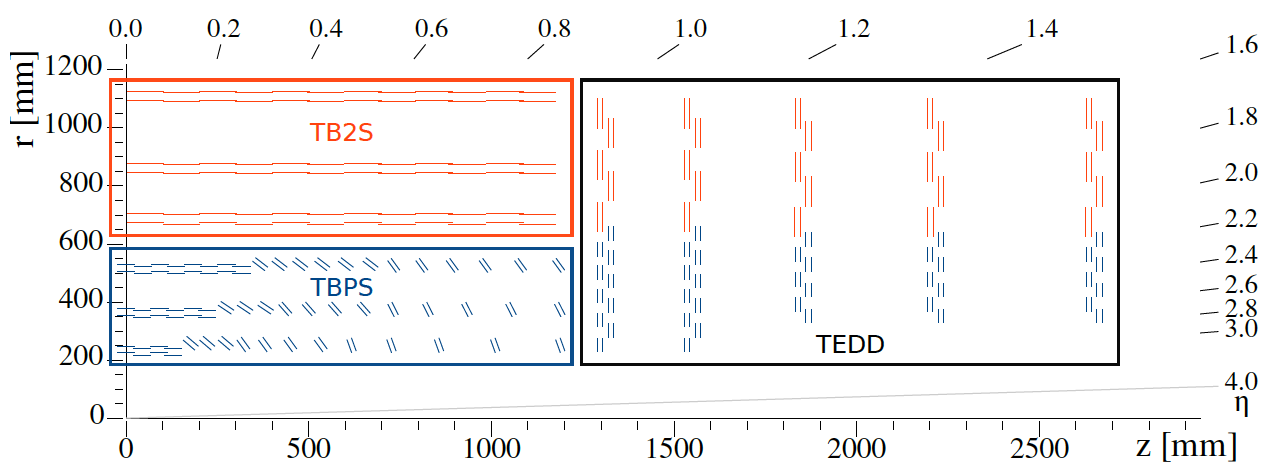
\includegraphics[width=.9\linewidth]{tex/Part2/fig/OT/OT-longitudinal.png}
\end{subfigure}
\begin{subfigure}
  \centering
  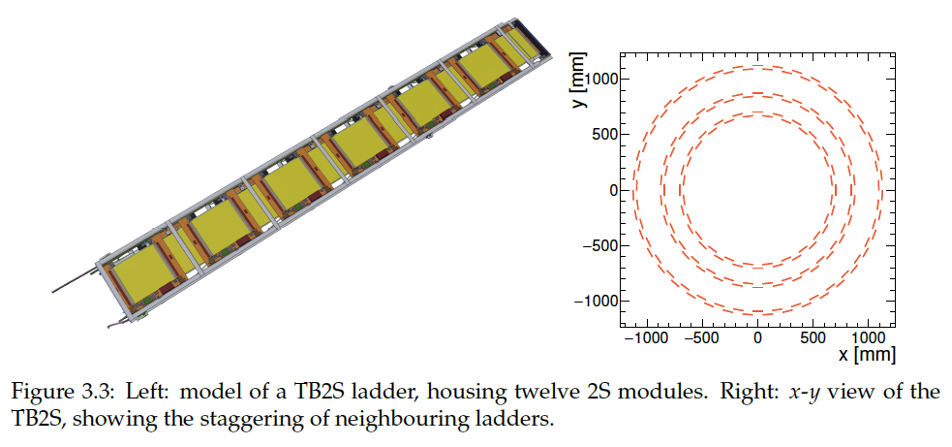
\includegraphics[width=.9\linewidth]{tex/Part2/fig/OT/OT-transverse.png}
\end{subfigure}
\caption{
  Layout of the CMS Phase II Outer Tracker.
  Top figure shows a longitudinal view with two regions in the barrel (TB2S, TBPS) and the endcap region (TEDD).
  Bottom figure shows a transverse view of the three TB2S layers (4, 5, and 6) and the layout of one ladder with 12 sensor modules.
  Track stubs from the  TB2S layer 6, with 78 ladders, will be used for luminosity measurement.  
}
\label{fig:OT_layout}
\end{figure}


\begin{figure}[hbtp]
\centering
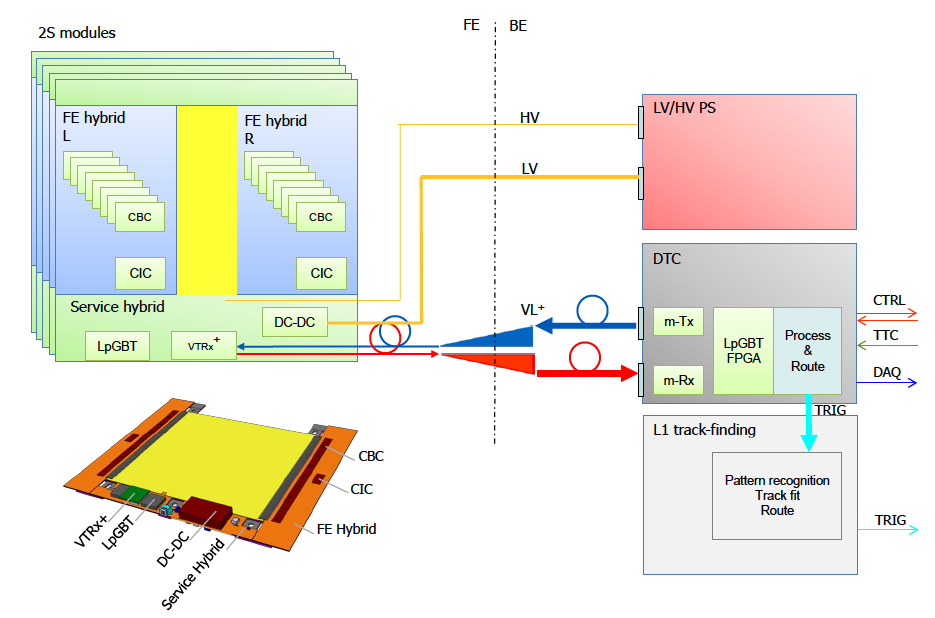
\includegraphics[width=.65\linewidth]{tex/Part2/fig/OT/OT-DAQoverview.png}
\caption{
  Design of the Phase II Outer Tracker frontend (FE) and backend (BE) electronics.   
}   
\label{fig:OT_DAQ}
\end{figure}


\begin{figure}[hbtp]
\centering
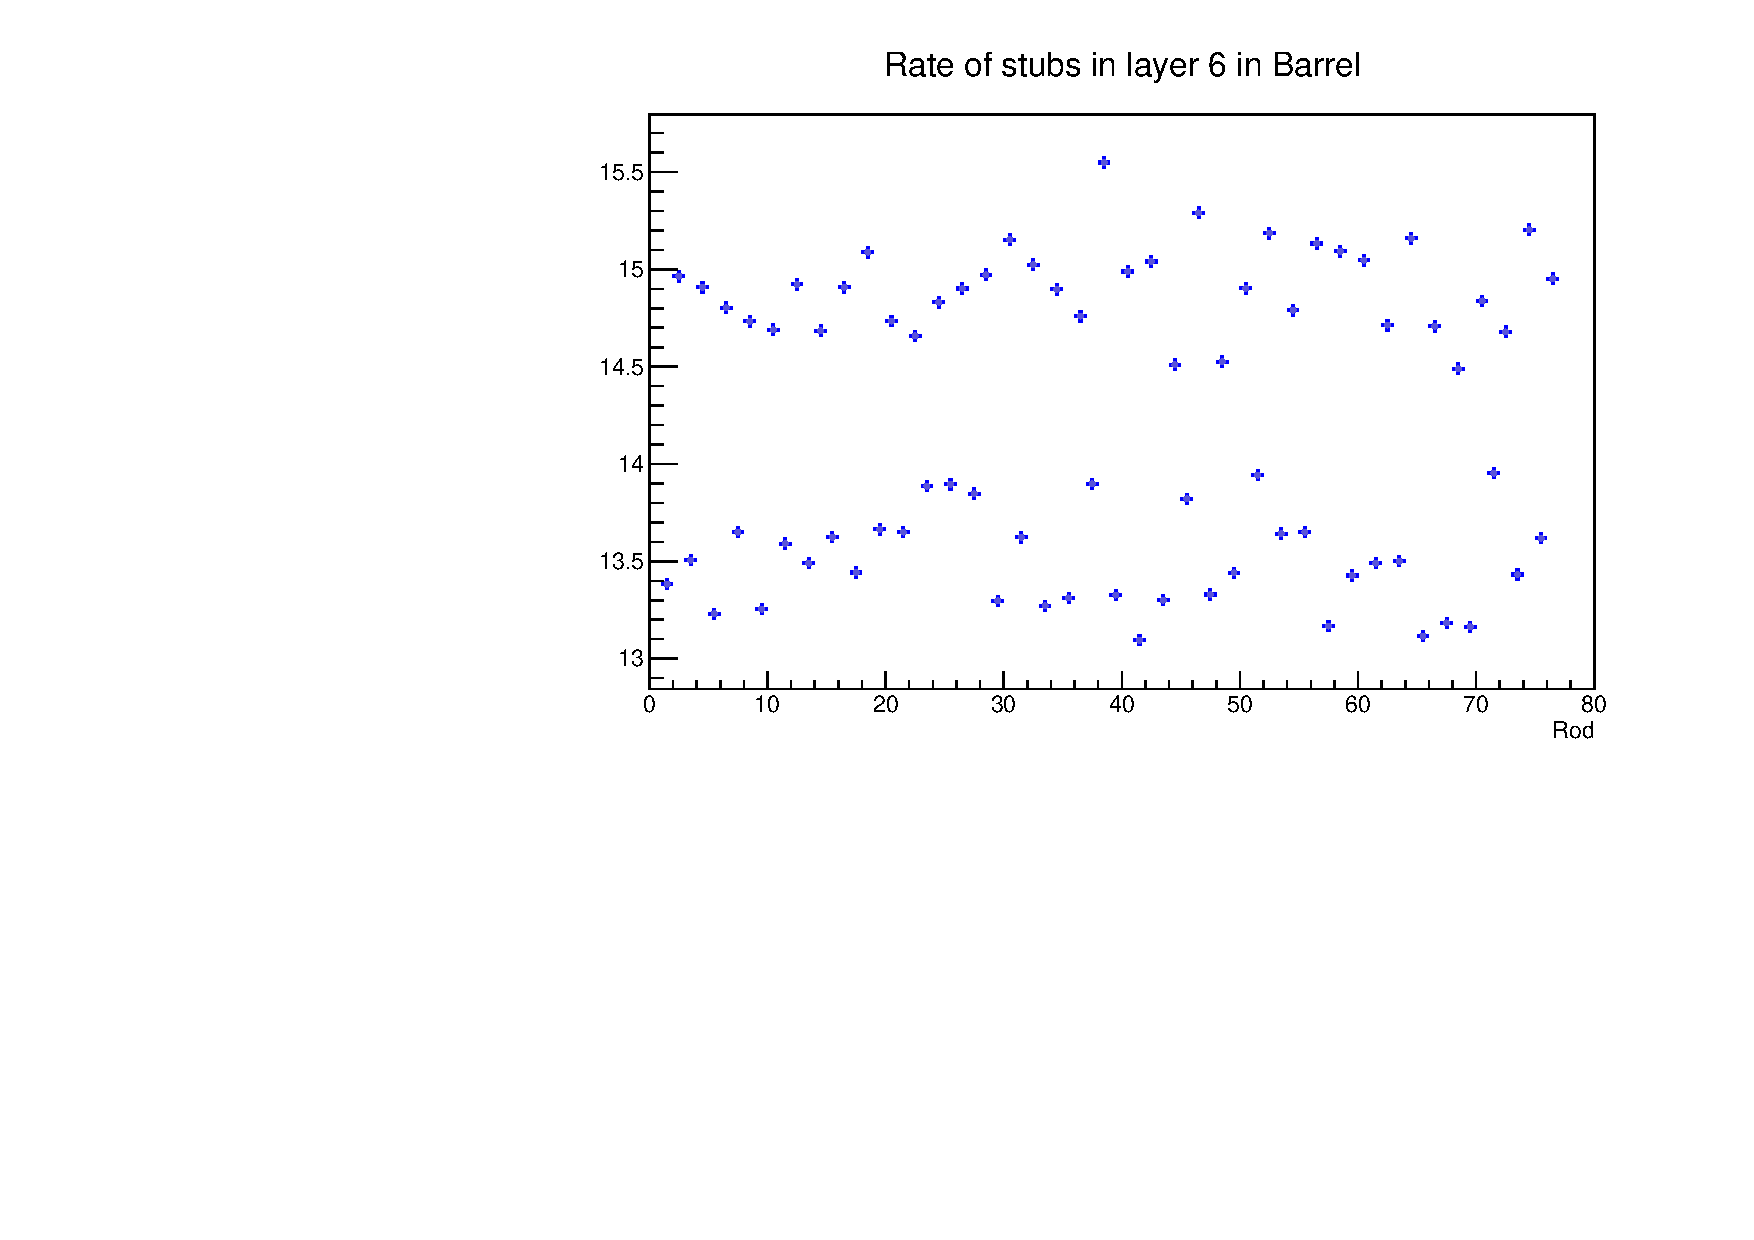
\includegraphics[width=.6\linewidth]{tex/Part2/fig/OT/OT-Rates.pdf}
\caption{
  Average number of track stubs per event per ladder as a function of the ladder id. The rate is determined from the CMS Phase II simulation for a pile-up of 200.
}
\label{fig:OT_rates}
\end{figure}


\begin{figure}[hbtp]
\centering
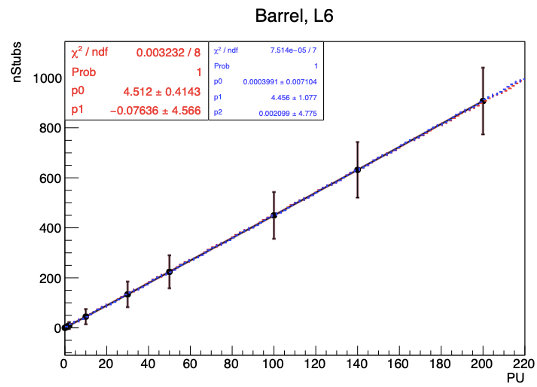
\includegraphics[width=.6\linewidth]{tex/Part2/fig/OT/OT-linearity.png}
\caption{
 Average number of track stubs per event as a function of pile-up determined from the CMS Phase II simulation showing a linear behaviour.
} 
\label{fig:OT_linearity}
\end{figure}
